\section{混合分布}
\label{sec:dfam-mixtures}

一批零件来自两条生产线，一条偏大、一条偏小，混在一起测量，直方图上会出现两个峰。单个高斯分布无论怎样平移伸缩都只有一个峰，推前一个固定的高斯也不自然。更直接的描述是照着来源写：先随机决定零件来自哪条线，再按那条线的规律产生尺寸。这样得到的分布族，参数分成两类：选择成分的规律，以及各成分自己的参数。

\subsection{有限混合}
\label{sec:dfam-finite-mixture}

设$P_1,\dots,P_m$是$\mathcal{X}$上的概率测度，$\bm{w}=(w_1,\dots,w_m)$是一张概率表。先抽成分指标$K$，$\mathbb{P}(K=k)=w_k$；再在$K=k$的条件下让$X\sim P_k$。由第~\ref{chap:conditional-distributions}章的全概率公式，
\[
  \begin{aligned}
    \mathbb{P}(X\in B)&=\sum_{k=1}^{m}\mathbb{P}(K=k)\,\mathbb{P}(X\in B\mid K=k)\\
    &=\sum_{k=1}^{m}w_kP_k(B).
  \end{aligned}
\]

\begin{definition}[有限混合]
\label{def:dfam-finite-mixture}
设$\bm{w}\in\Delta_{m-1}$，$P_1,\dots,P_m\in\mathcal{P}(\mathcal{X})$。概率测度
\begin{equation}
  P=\sum_{k=1}^{m}w_kP_k
  \label{eq:dfam-finite-mixture}
\end{equation}
称为成分$P_1,\dots,P_m$以\term{混合权重}（mixture weights）$\bm{w}$构成的\term{有限混合}（finite mixture）。若各成分取自一个参数化族，$P_k=Q_{\bm{\eta}_k}$，则混合族的参数是$(\bm{w},\bm{\eta}_1,\dots,\bm{\eta}_m)$。
\end{definition}

式~\eqref{eq:dfam-finite-mixture}是概率的加权平均，对每个事件逐一成立。所以分布函数、密度（若各成分相对同一个$\nu$有密度$p_k$）和有限的期望都按同样的权重相加：
\[
  F=\sum_kw_kF_k,\qquad p=\sum_kw_kp_k,\qquad\mathbb{E}_P[g]=\sum_kw_k\,\mathbb{E}_{P_k}[g].
\]
分位数不在其列。分位数函数是分布函数的广义逆，逆运算与加权平均不能交换，混合的中位数一般不等于各成分中位数的加权平均。

\paragraph{均值与方差}
设第$k$个成分的均值与方差为$m_k$、$s_k^{2}$，记$\bar{m}=\sum_kw_km_k$。由上式，$\mathbb{E}[X]=\bar{m}$。方差由全方差公式（第~\ref{chap:conditional-expectation}章）给出，其中两个条件量是
\[
  \mathbb{E}[X\mid K]=m_K,\qquad\operatorname{Var}(X\mid K)=s_K^{2},
\]
代入得到
\begin{equation}
  \operatorname{Var}(X)=\sum_{k}w_ks_k^{2}+\sum_kw_k(m_k-\bar{m})^{2}.
  \label{eq:dfam-mixture-variance}
\end{equation}
第一项是成分内部的平均波动，第二项是成分中心之间的分散。若把各成分看成放在$m_k$处的质量块，第二项正是这组质量块绕总重心的转动惯量。

\paragraph{两个高斯成分}
取等权的两个成分$\mathcal{N}(-a,1)$与$\mathcal{N}(a,1)$，$a>0$，混合密度是
\[
  f_a(x)=\tfrac12\varphi(x+a)+\tfrac12\varphi(x-a).
\]
由式~\eqref{eq:dfam-mixture-variance}，均值是$0$，方差是$1+a^{2}$。取$a=1.5$，方差是$3.25$，比每个成分的方差$1$大得多，多出的$2.25$全部来自两个中心的分离。

$f_a$关于$0$对称，所以$f_a'(0)=0$。要判断$0$处是峰还是谷，看二阶导数。$\varphi'(z)=-z\varphi(z)$，再求一次导，
\[
  \varphi''(z)=(z^{2}-1)\varphi(z).
\]
代入$f_a$，两项在$x=0$处相等，得到
\begin{equation}
  f_a''(0)=(a^{2}-1)\,\varphi(a).
  \label{eq:dfam-mixture-curvature}
\end{equation}

$a<1$时$f_a''(0)<0$，中心是局部极大；$a>1$时$f_a''(0)>0$，中心变成局部极小。后一种情形下$f_a$在$0$处是谷，又在$\pm\infty$处趋于零，所以两侧各有一个峰，密度至少有两个峰。$a=1$是转折点，两个成分中心相距$2$，恰为成分标准差的两倍。图~\ref{fig:dfam-mixture-separation}画出$a=0.5,1,1.5,2$的情形。

\begin{BookInlineFigure}
  \centering
  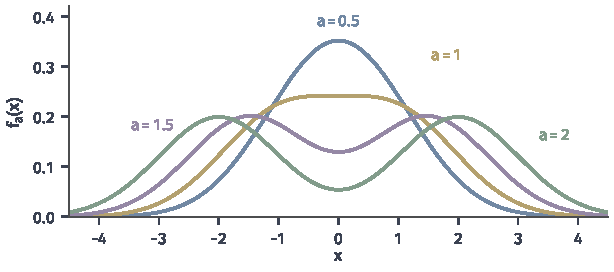
\includegraphics[width=104mm]{figures/07-probability/04-distribution-analysis/matplotlib/dfam-mixture-separation/figure.pdf}
  \caption{等权混合$\frac12\mathcal{N}(-a,1)+\frac12\mathcal{N}(a,1)$的密度，$a=0.5$（蓝）、$1$（黄）、$1.5$（紫）、$2$（绿）。$a=1$时中心处的二阶导数为零，顶部最平；$a>1$时中心是谷，出现两个峰。}
  \label{fig:dfam-mixture-separation}
\end{BookInlineFigure}

单个高斯分布的密度从中心向两侧单调下降，只有一个峰；$\mathcal{N}(0,1)$生成的位置尺度族中所有成员都是如此。两个高斯的混合却能有两个峰。这是混合族比它的成分族多出来的形状。

\paragraph{只改权重与改变成分}
混合族的两类参数作用不同。固定成分只改权重，密度$p=\sum_kw_kp_k$对$\bm{w}$是线性的：权重把质量在几块固定的形状之间重新分配，峰的位置大体不动，峰的高低此消彼长。全体权重给出的分布构成一个凸集，第~\ref{sec:dfam-candidates}节三角形中的线段就是两个概率表的全部混合。

改变成分参数则改变形状本身，密度对它们是非线性的。图~\ref{fig:dfam-mixture-weights-params}(a)固定$a=1.5$，把第二个成分的权重从$0.5$增到$0.9$，右峰升高、左峰缩成肩部；(b)固定等权，把第二个成分的标准差缩小到$0.5$、中心移到$2$，右峰变得又窄又高，左峰的形状不变。

\begin{BookInlineFigure}
  \centering
  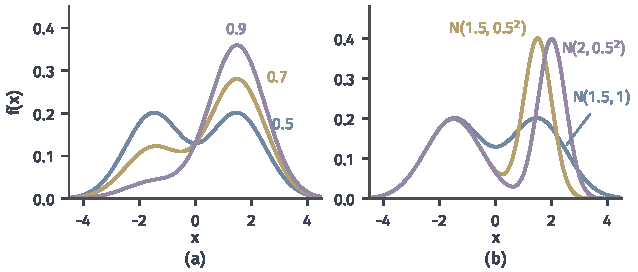
\includegraphics[width=108mm]{figures/07-probability/04-distribution-analysis/matplotlib/dfam-mixture-weights-params/figure.pdf}
  \caption{混合族中两类参数的作用。(a)成分固定为$\mathcal{N}(-1.5,1)$与$\mathcal{N}(1.5,1)$，第二个成分的权重为$0.5$（蓝）、$0.7$（黄）、$0.9$（紫）。(b)等权，第二个成分为$\mathcal{N}(1.5,1)$（蓝）、$\mathcal{N}(1.5,0.5^{2})$（黄）、$\mathcal{N}(2,0.5^{2})$（紫）；第一个成分始终是$\mathcal{N}(-1.5,1)$。}
  \label{fig:dfam-mixture-weights-params}
\end{BookInlineFigure}

\paragraph{混合不是取值的平均}
“按权重$\tfrac12,\tfrac12$组合两个随机量”有两种截然不同的意思。设$Y_1\sim\mathcal{N}(-1.5,1)$与$Y_2\sim\mathcal{N}(1.5,1)$独立。混合是以概率$\tfrac12$报告$Y_1$、以概率$\tfrac12$报告$Y_2$，分布是$f_{1.5}$，方差$3.25$。取值的平均$\tfrac12Y_1+\tfrac12Y_2$则是两个独立高斯的线性组合，由第~\ref{chap:multivariate-distributions}章，它服从
\[
  \mathcal{N}\bigl(0,\ \tfrac14+\tfrac14\bigr)=\mathcal{N}(0,0.5).
\]
它只有一个峰，方差只有$0.5$。

两者的差别在于加权的对象。混合对概率加权，每次只取一个成分的值，两个峰都保留下来；取值平均对随机变量加权，每次都把两个值折中，正负偏离互相抵消。图~\ref{fig:dfam-mix-vs-sum}并排画出两者。

\begin{BookInlineFigure}
  \centering
  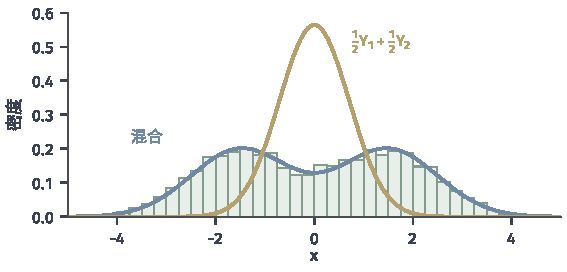
\includegraphics[width=96mm]{figures/07-probability/04-distribution-analysis/matplotlib/dfam-mix-vs-sum/figure.pdf}
  \caption{同一对成分$\mathcal{N}(-1.5,1)$、$\mathcal{N}(1.5,1)$的两种“等权组合”。蓝线是混合$\frac12\mathcal{N}(-1.5,1)+\frac12\mathcal{N}(1.5,1)$，方差$3.25$；黄线是独立变量的平均$\frac12Y_1+\frac12Y_2\sim\mathcal{N}(0,0.5)$。绿色直方图是混合的$5000$个模拟样本（种子$716$）。}
  \label{fig:dfam-mix-vs-sum}
\end{BookInlineFigure}

\subsection{连续混合}
\label{sec:dfam-continuous-mixture}

有限混合的成分指标只取有限个值。若影响结果的隐藏因素是连续的，例如每个零件的加工精度都略有不同，就要让成分由一个连续变量$S$索引。给定$S=s$时，$X$的条件分布是$K(s,\cdot)$；$S$本身服从分布$M$。

\begin{definition}[一般混合]
\label{def:dfam-general-mixture}
设$(\mathcal{S},\mathcal{F}_{\mathcal{S}})$上有概率测度$M$，$K$是从$\mathcal{S}$到$\mathcal{X}$的概率核。概率测度
\begin{equation}
  P(B)=\int_{\mathcal{S}}K(s,B)\,M(\mathrm{d}s),\qquad B\in\mathcal{F}_{\mathcal{X}},
  \label{eq:dfam-general-mixture}
\end{equation}
称为核$K$以\term{混合测度}（mixing measure）$M$构成的混合。$M$不是离散分布时，常称为\term{连续混合}（continuous mixture）。
\end{definition}

$P$确实是概率测度：$K(s,\mathcal{X})=1$给出$P(\mathcal{X})=1$；对互不相交的$B_1,B_2,\dots$，$K(s,\cdot)$可数可加，再由单调收敛定理交换求和与积分，得到$P$可数可加。式~\eqref{eq:dfam-general-mixture}正是第~\ref{chap:conditional-distributions}章由边缘分布与条件分布恢复$X$的边缘分布的公式，这里把它反过来用作构造。取$M=\sum_kw_k\delta_k$，积分退回求和，得到式~\eqref{eq:dfam-finite-mixture}。

若每个$K(s,\cdot)$相对同一个$\nu$有密度$k(x\mid s)$，且$k$对$(s,x)$联合可测，则由Tonelli定理交换积分次序，
\[
  P(B)=\int_{\mathcal{S}}\int_Bk(x\mid s)\,\nu(\mathrm{d}x)\,M(\mathrm{d}s)=\int_B\Bigl(\int_{\mathcal{S}}k(x\mid s)\,M(\mathrm{d}s)\Bigr)\nu(\mathrm{d}x).
\]
所以混合的密度是条件密度按$M$的平均：
\begin{equation}
  p(x)=\int_{\mathcal{S}}k(x\mid s)\,M(\mathrm{d}s).
  \label{eq:dfam-mixture-density}
\end{equation}

\paragraph{正态尺度混合}
最常用的连续混合是第~\ref{chap:multivariate-distributions}章的正态尺度混合：$W\geq0$与$Z\sim\mathcal{N}(0,1)$独立，$X=\sqrt{W}Z$。给定$W=w$，$X\sim\mathcal{N}(0,w)$，混合测度是$W$的分布。那一章用它构造了t分布与Laplace分布；这里关心的是，不管$W$怎样分布，混合都带来什么共同的形状。

\begin{theorem}[尺度混合使峰度不小于三]
\label{thm:dfam-scale-mixture-kurtosis}
设$W\geq0$，$\mathbb{E}[W^{2}]<\infty$，$\mathbb{P}(W>0)>0$，$Z\sim\mathcal{N}(0,1)$与$W$独立，$X=\sqrt{W}Z$。则$X$的峰度
\begin{equation}
  \kappa(X)=\frac{\mathbb{E}[X^{4}]}{(\mathbb{E}[X^{2}])^{2}}=\frac{3\,\mathbb{E}[W^{2}]}{(\mathbb{E}[W])^{2}}\geq3 ,
  \label{eq:dfam-scale-kurtosis}
\end{equation}
等号成立当且仅当$W$几乎必然为常数。
\end{theorem}

\begin{proof}
$X$的均值是$\mathbb{E}[\sqrt{W}]\,\mathbb{E}[Z]=0$。由独立性与$\mathbb{E}[Z^{2}]=1$、$\mathbb{E}[Z^{4}]=3$，
\[
  \mathbb{E}[X^{2}]=\mathbb{E}[W]\,\mathbb{E}[Z^{2}]=\mathbb{E}[W],\qquad\mathbb{E}[X^{4}]=\mathbb{E}[W^{2}]\,\mathbb{E}[Z^{4}]=3\,\mathbb{E}[W^{2}].
\]
由$\mathbb{P}(W>0)>0$，$\mathbb{E}[W]>0$，比值有意义。由方差非负，
\[
  \mathbb{E}[W^{2}]-(\mathbb{E}[W])^{2}=\operatorname{Var}(W)\geq0 ,
\]
所以$\kappa(X)\geq3$；等号成立当且仅当$\operatorname{Var}(W)=0$，即$W$几乎必然等于常数。
\end{proof}

高斯分布的峰度恰好是$3$。定理说，只要尺度真的随机，混合的峰度就严格大于$3$：大的$W$贡献远处的值，小的$W$贡献贴近$0$的值，结果比同方差的高斯分布中间更尖、尾部更厚。例如$W$以各$\tfrac12$的概率取$0.5$和$1.5$，这是两成分的有限混合，
\[
  \mathbb{E}[W]=1,\qquad\mathbb{E}[W^{2}]=\tfrac12(0.25+2.25)=1.25,\qquad\kappa(X)=3.75 .
\]
取$W\sim\operatorname{Exp}(1)$，$\mathbb{E}[W]=1$，$\mathbb{E}[W^{2}]=2$，由式~\eqref{eq:dfam-scale-kurtosis}得$\kappa(X)=6$；第~\ref{chap:multivariate-distributions}章算出这时$X$服从$\operatorname{Laplace}(0,1/\sqrt2)$，其峰度正是$6$。

\paragraph{共同尺度带来的依赖}
在多元情形，同一个$W$乘到所有分量上。设$\bm{Z}\sim\mathcal{N}(\bm{0},\bm{I}_2)$与$W$独立，$\bm{X}=\sqrt{W}\bm{Z}$，$\mathbb{E}[W^{2}]<\infty$。由独立性，
\[
  \operatorname{Cov}(\bm{X})=\mathbb{E}[W]\,\bm{I}_2 ,
\]
两个分量不相关。但它们不独立：
\[
  \mathbb{E}[X_1^{2}X_2^{2}]=\mathbb{E}[W^{2}]\,\mathbb{E}[Z_1^{2}]\,\mathbb{E}[Z_2^{2}]=\mathbb{E}[W^{2}],
\]
而两个边缘二阶矩的乘积是
\[
  \mathbb{E}[X_1^{2}]\,\mathbb{E}[X_2^{2}]=(\mathbb{E}[W])^{2}.
\]
若$W$不是常数，两者不等，$X_1^{2}$与$X_2^{2}$正相关，所以$X_1,X_2$不独立。$W\sim\operatorname{Exp}(1)$时
\[
  \operatorname{Cov}(X_1^{2},X_2^{2})=\mathbb{E}[W^{2}]-(\mathbb{E}[W])^{2}=1 .
\]

直观上，$W$大的那一次，两个分量同时被放大；$W$小的那一次，两个分量同时贴近原点。图~\ref{fig:dfam-scale-mixture}(b)中，离原点较远的点（红）均匀地散在各个方向上，包括对角方向，说明两个分量常常一起取大值；(c)让每个分量各用一个独立的$W_i$，边缘分布与(b)完全相同，远处的点却集中在两条坐标轴附近：一个分量很大时，另一个分量通常仍然不大。只看边缘分布或协方差，分不出这两种模型。

\begin{BookInlineFigure}
  \centering
  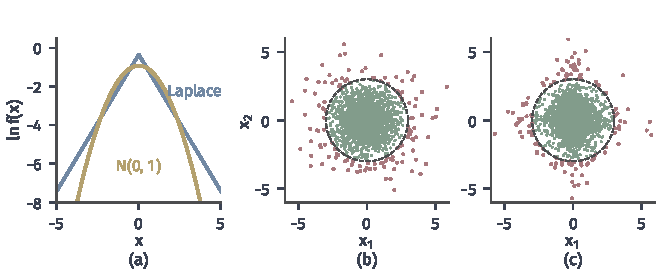
\includegraphics[width=112mm]{figures/07-probability/04-distribution-analysis/matplotlib/dfam-scale-mixture/figure.pdf}
  \caption{正态尺度混合，$W\sim\operatorname{Exp}(1)$。(a)一元密度的对数：$X=\sqrt{W}Z$即$\operatorname{Laplace}(0,1/\sqrt2)$（蓝），与同方差的$\mathcal{N}(0,1)$（黄）；混合的中心更尖、尾部按直线而非抛物线下降。(b)共同尺度$\sqrt{W}(Z_1,Z_2)$的$3000$个样本。(c)独立尺度$(\sqrt{W_1}Z_1,\sqrt{W_2}Z_2)$的$3000$个样本。(b)(c)中深灰虚线是半径$3$的圆，圆外的点标红；两图的边缘分布相同，协方差都是$\bm{I}_2$；模拟种子$716$。}
  \label{fig:dfam-scale-mixture}
\end{BookInlineFigure}

\paragraph{计数的混合}
连续混合同样适用于离散结果。设给定$\Lambda=\lambda$时$X\sim\operatorname{Poisson}(\lambda)$，而强度$\Lambda\sim\operatorname{Gamma}(\alpha,\beta)$。由式~\eqref{eq:dfam-mixture-density}，以计数测度为参考，
\[
  \mathbb{P}(X=k)=\int_0^\infty\mathrm{e}^{-\lambda}\frac{\lambda^{k}}{k!}\cdot\frac{\beta^{\alpha}\lambda^{\alpha-1}\mathrm{e}^{-\beta\lambda}}{\Gamma(\alpha)}\,\mathrm{d}\lambda .
\]

把$\lambda$的幂与指数合并，剩下的积分是一个Gamma积分，
\[
  \int_0^\infty\lambda^{k+\alpha-1}\mathrm{e}^{-(1+\beta)\lambda}\,\mathrm{d}\lambda=\frac{\Gamma(k+\alpha)}{(1+\beta)^{k+\alpha}} .
\]
代回得到
\begin{equation}
  \mathbb{P}(X=k)=\frac{\Gamma(k+\alpha)}{k!\,\Gamma(\alpha)}\Bigl(\frac{\beta}{1+\beta}\Bigr)^{\alpha}\Bigl(\frac{1}{1+\beta}\Bigr)^{k},\qquad k=0,1,\dots
  \label{eq:dfam-negative-binomial}
\end{equation}
这是\term{负二项分布}（negative binomial distribution）。

取$\alpha=2$、$\beta=1$，式~\eqref{eq:dfam-negative-binomial}化为$\mathbb{P}(X=k)=(k+1)/2^{k+2}$，前几项是
\[
  p_0=\tfrac14,\quad p_1=\tfrac14,\quad p_2=\tfrac{3}{16},\quad p_3=\tfrac18 .
\]
均值由全期望公式得$\mathbb{E}[\Lambda]=\alpha/\beta=2$，与$\operatorname{Poisson}(2)$相同。方差由全方差公式得
\[
  \operatorname{Var}(X)=\mathbb{E}[\Lambda]+\operatorname{Var}(\Lambda)=\frac{\alpha}{\beta}+\frac{\alpha}{\beta^{2}}=4 ,
\]
是$\operatorname{Poisson}(2)$方差的两倍。强度的随机性使$0$和大计数都更常见：$p_0=0.25$，而$\operatorname{Poisson}(2)$在$0$处只有$\mathrm{e}^{-2}\approx0.135$，见图~\ref{fig:dfam-poisson-gamma}。

\begin{BookInlineFigure}
  \centering
  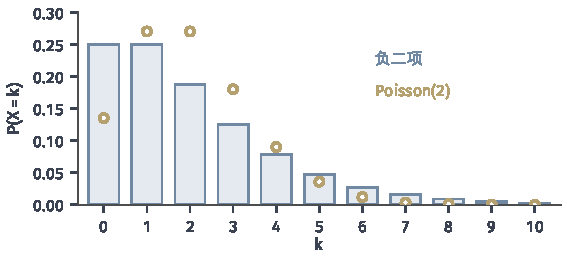
\includegraphics[width=96mm]{figures/07-probability/04-distribution-analysis/matplotlib/dfam-poisson-gamma/figure.pdf}
  \caption{计数的连续混合。浅蓝柱是$\operatorname{Poisson}(\Lambda)$、$\Lambda\sim\operatorname{Gamma}(2,1)$的混合，即负二项分布$(k+1)/2^{k+2}$；黄色空心点是同均值的$\operatorname{Poisson}(2)$。两者均值都是$2$，方差分别为$4$与$2$。}
  \label{fig:dfam-poisson-gamma}
\end{BookInlineFigure}

\paragraph{改变混合测度与改变核}
连续混合族有两个可以变动的部分。固定核$K(w,\cdot)=\mathcal{N}(0,w)$，让混合测度$M$取遍$(0,\infty)$上全体概率测度，得到全体正态尺度混合。这个族是凸的，包含所有t分布与上面的Laplace分布，远比任何有限维族大；但它的成员都关于$0$对称，由定理~\ref{thm:dfam-scale-mixture-kurtosis}，四阶矩有限的成员峰度都不小于$3$。

所以改变$M$无论怎样都造不出偏斜的分布，也造不出比高斯更“平”的分布。$\operatorname{Unif}(-\sqrt3,\sqrt3)$的方差为$1$，峰度为$1.8$，它就不是任何正态尺度混合。要得到这些形状，必须换掉核：例如把$\mathcal{N}(0,w)$换成$\mathcal{N}(s,1)$，让混合测度作用在位置上，或者像Poisson–Gamma那样换成离散的核。混合测度决定成分怎样搭配，核决定可以搭配的成分是什么形状。

\subsection{混合表示的非唯一性}
\label{sec:dfam-mixture-nonuniqueness}

混合族的参数比分布多出很多冗余。第~\ref{sec:dfam-identifiability}节已经看到标签置换；这里把各种冗余列清楚，再说明成分互相重叠并不是冗余。

\paragraph{冗余从哪里来}
考虑等方差的两成分高斯混合
\[
  P_{(w,\mu_1,\mu_2)}=w\,\mathcal{N}(\mu_1,1)+(1-w)\,\mathcal{N}(\mu_2,1),\qquad 0\leq w\leq1 .
\]
第一种冗余是标签置换：$(w,\mu_1,\mu_2)$与$(1-w,\mu_2,\mu_1)$给出同一个分布。它把参数成对地粘在一起，每个真正的两成分分布恰好对应两组参数。

第二种冗余来自重复成分。$\mu_1=\mu_2=\mu$时，两个成分相同，
\[
  w\,\mathcal{N}(\mu,1)+(1-w)\,\mathcal{N}(\mu,1)=\mathcal{N}(\mu,1)
\]
对每个$w\in[0,1]$成立，权重完全看不见。第三种冗余来自零权重：$w=0$时，$\mu_1$不出现在分布中，可以取任意值。

以$\mathcal{N}(0,1)$为例，它的全部表示是
\[
  \{w\in[0,1],\ \mu_1=\mu_2=0\}\cup\{w=0,\ \mu_2=0\}\cup\{w=1,\ \mu_1=0\}.
\]
这是参数空间中的三条线段（其中两条是整条直线），不再是孤立的点。图~\ref{fig:dfam-mixture-fibers}(a)在$\mu_2=0$的截面上画出其中两条：$\mu_1=0$的竖线与$w=0$的横线交成一个十字。

\begin{BookInlineFigure}
  \centering
  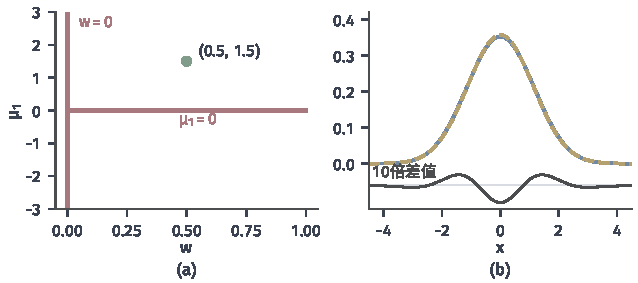
\includegraphics[width=108mm]{figures/07-probability/04-distribution-analysis/matplotlib/dfam-mixture-fibers/figure.pdf}
  \caption{混合表示的冗余与重叠。(a)$\mu_2=0$的截面$(w,\mu_1)$中，给出$\mathcal{N}(0,1)$的参数（红线）：$\mu_1=0$时任何$w$都可以，$w=0$时任何$\mu_1$都可以；绿点是$(0.5,1.5)$，代表一个真正的两成分混合，它在这个截面上只出现一次。(b)重叠很大的混合$\frac12\mathcal{N}(-0.5,1)+\frac12\mathcal{N}(0.5,1)$（蓝）与同均值、同方差的$\mathcal{N}(0,1.25)$（黄）；下方深灰线是两者密度之差，放大$10$倍。}
  \label{fig:dfam-mixture-fibers}
\end{BookInlineFigure}

\paragraph{重叠不等于不可辨识}
成分互相重叠是另一回事。$\tfrac12\mathcal{N}(-0.5,1)+\tfrac12\mathcal{N}(0.5,1)$的两个成分大部分重合，混合只有一个峰，看上去几乎就是一个高斯：图~\ref{fig:dfam-mixture-fibers}(b)中它与同均值同方差的$\mathcal{N}(0,1.25)$的密度之差最大不到$0.005$，约为峰高的$1.4\%$。但两者是不同的分布，而且下面的定理说明，这个混合的参数除了标签置换外是唯一确定的。

记$\varphi_\sigma(x)=\varphi(x/\sigma)/\sigma$为$\mathcal{N}(0,\sigma^{2})$的密度。证明要用到一个关于指数函数的事实。

\begin{lemma}[不同指数的指数函数线性无关]
\label{lem:dfam-exp-independent}
设$\nu_1>\nu_2>\cdots>\nu_r$为实数，$c_1,\dots,c_r$为实数。若对一切$t\in\mathbb{R}$有$\sum_{j=1}^{r}c_j\mathrm{e}^{\nu_jt}=0$，则$c_1=\cdots=c_r=0$。
\end{lemma}

\begin{proof}
两边乘以$\mathrm{e}^{-\nu_1t}$，得
\[
  c_1+\sum_{j=2}^{r}c_j\mathrm{e}^{(\nu_j-\nu_1)t}=0 .
\]
各$\nu_j-\nu_1<0$，令$t\to+\infty$，求和项趋于零，所以$c_1=0$。对剩下的$r-1$项重复这一步，依次得到$c_2=\cdots=c_r=0$。
\end{proof}

\begin{theorem}[已知方差的高斯位置混合可辨识]
\label{thm:dfam-gaussian-mixture-identifiable}
固定$\sigma>0$。设$\mu_1,\dots,\mu_m$互不相同，$\mu'_1,\dots,\mu'_{m'}$互不相同，权重$w_k>0$、$w'_l>0$且各自和为$1$。若
\begin{equation}
  \sum_{k=1}^{m}w_k\,\mathcal{N}(\mu_k,\sigma^{2})=\sum_{l=1}^{m'}w'_l\,\mathcal{N}(\mu'_l,\sigma^{2}),
  \label{eq:dfam-mixture-equal}
\end{equation}
则$m=m'$，且存在$\{1,\dots,m\}$的置换$\pi$，使$\mu'_{\pi(k)}=\mu_k$、$w'_{\pi(k)}=w_k$。
\end{theorem}

\begin{proof}
两边是同一个分布，所以对一切$t$，$\mathrm{e}^{tX}$在两边的期望相同。$\mathcal{N}(\mu,\sigma^{2})$的矩母函数是$\mathrm{e}^{\mu t+\sigma^{2}t^{2}/2}$，有限混合的矩母函数是成分矩母函数的加权和，于是
\[
  \mathrm{e}^{\sigma^{2}t^{2}/2}\sum_{k}w_k\mathrm{e}^{\mu_kt}=\mathrm{e}^{\sigma^{2}t^{2}/2}\sum_{l}w'_l\mathrm{e}^{\mu'_lt},\qquad t\in\mathbb{R}.
\]
约去公共因子$\mathrm{e}^{\sigma^{2}t^{2}/2}>0$，移项，
\[
  \sum_{k}w_k\mathrm{e}^{\mu_kt}-\sum_lw'_l\mathrm{e}^{\mu'_lt}=0,\qquad t\in\mathbb{R}.
\]

把两组位置合在一起，按不同的值合并同类项。对每个出现过的值$\nu$，它的系数是“$\nu$在左边的权重”减去“$\nu$在右边的权重”，在一边没有出现时那一边记为零。由引理~\ref{lem:dfam-exp-independent}，每个系数都为零。若某个$\mu_k$不在右边出现，它的系数就是$w_k>0$，矛盾；所以每个$\mu_k$都等于某个$\mu'_l$，且权重相同。对右边同样论证，两组位置作为集合相同，于是$m=m'$，对应的权重相等。
\end{proof}

定理的条件都有作用。位置互不相同、权重为正，排除了重复成分与零权重两种冗余；结论中的置换$\pi$就是标签置换，它无法消除。方差$\sigma^{2}$固定已知也很关键：它让公共因子$\mathrm{e}^{\sigma^{2}t^{2}/2}$可以约去。

\paragraph{成分族决定能否识别}
可辨识的条件要按所用的成分族逐一核对，不能从高斯推到别的族。Bernoulli成分是最极端的反例：对任意$w,a,b\in[0,1]$，
\[
  w\operatorname{Bern}(a)+(1-w)\operatorname{Bern}(b)=\operatorname{Bern}\bigl(wa+(1-w)b\bigr).
\]
无论成分怎样分开，混合仍是一个Bernoulli分布，只有一个数$wa+(1-w)b$可见，三个参数中有两个完全无法确定。均匀成分也有类似现象：
\[
  \tfrac12\operatorname{Unif}(0,1)+\tfrac12\operatorname{Unif}(1,2)=\operatorname{Unif}(0,2),
\]
一个两成分表示与一个单成分表示给出同一个分布。

这两个例子与高斯的差别不在于成分是否重叠，均匀的例子中两个成分根本不重叠。差别在于成分族本身在混合下是否“封闭”：Bernoulli族的混合仍在Bernoulli族里，均匀分布可以切成更小的均匀分布再拼回去。高斯成分做不到这一点，定理~\ref{thm:dfam-gaussian-mixture-identifiable}的证明正是利用了矩母函数中不同的指数无法互相抵消。
